\documentclass[12pt]{article}
\usepackage[margin=1in]{geometry}
\usepackage{pythontex}
\usepackage{tabularx}
\usepackage{graphicx}
\usepackage{titling}
\usepackage{amsmath}
\usepackage{ragged2e}
\usepackage{float}
\usepackage[style=apa, backend=biber]{biblatex}
\usepackage{minted}
\usepackage[font=small,labelfont=bf]{caption}

\addbibresource{ia.bib}

\title{Using Machine Learning to Predict Typing Speed}
\author{jjr117}
\date{}

\newcommand{\code}[1]{\texttt{#1}}

\newenvironment{textexamples}
  {\medskip\par\setlength{\parindent}{0pt}}
  {\par\medskip}

\graphicspath{{assets/}}

\begin{document}

\maketitle

\section*{Introduction}

One of my hobbies is competitive typing, where I compete with my friends to type a text as quickly as possible. We often use a website called TypeRacer, where your goal is to drive a racecar to the finish line, and the position of your racecar is determined by how many words you've typed correctly in a certain text:

\begin{figure}[H]
	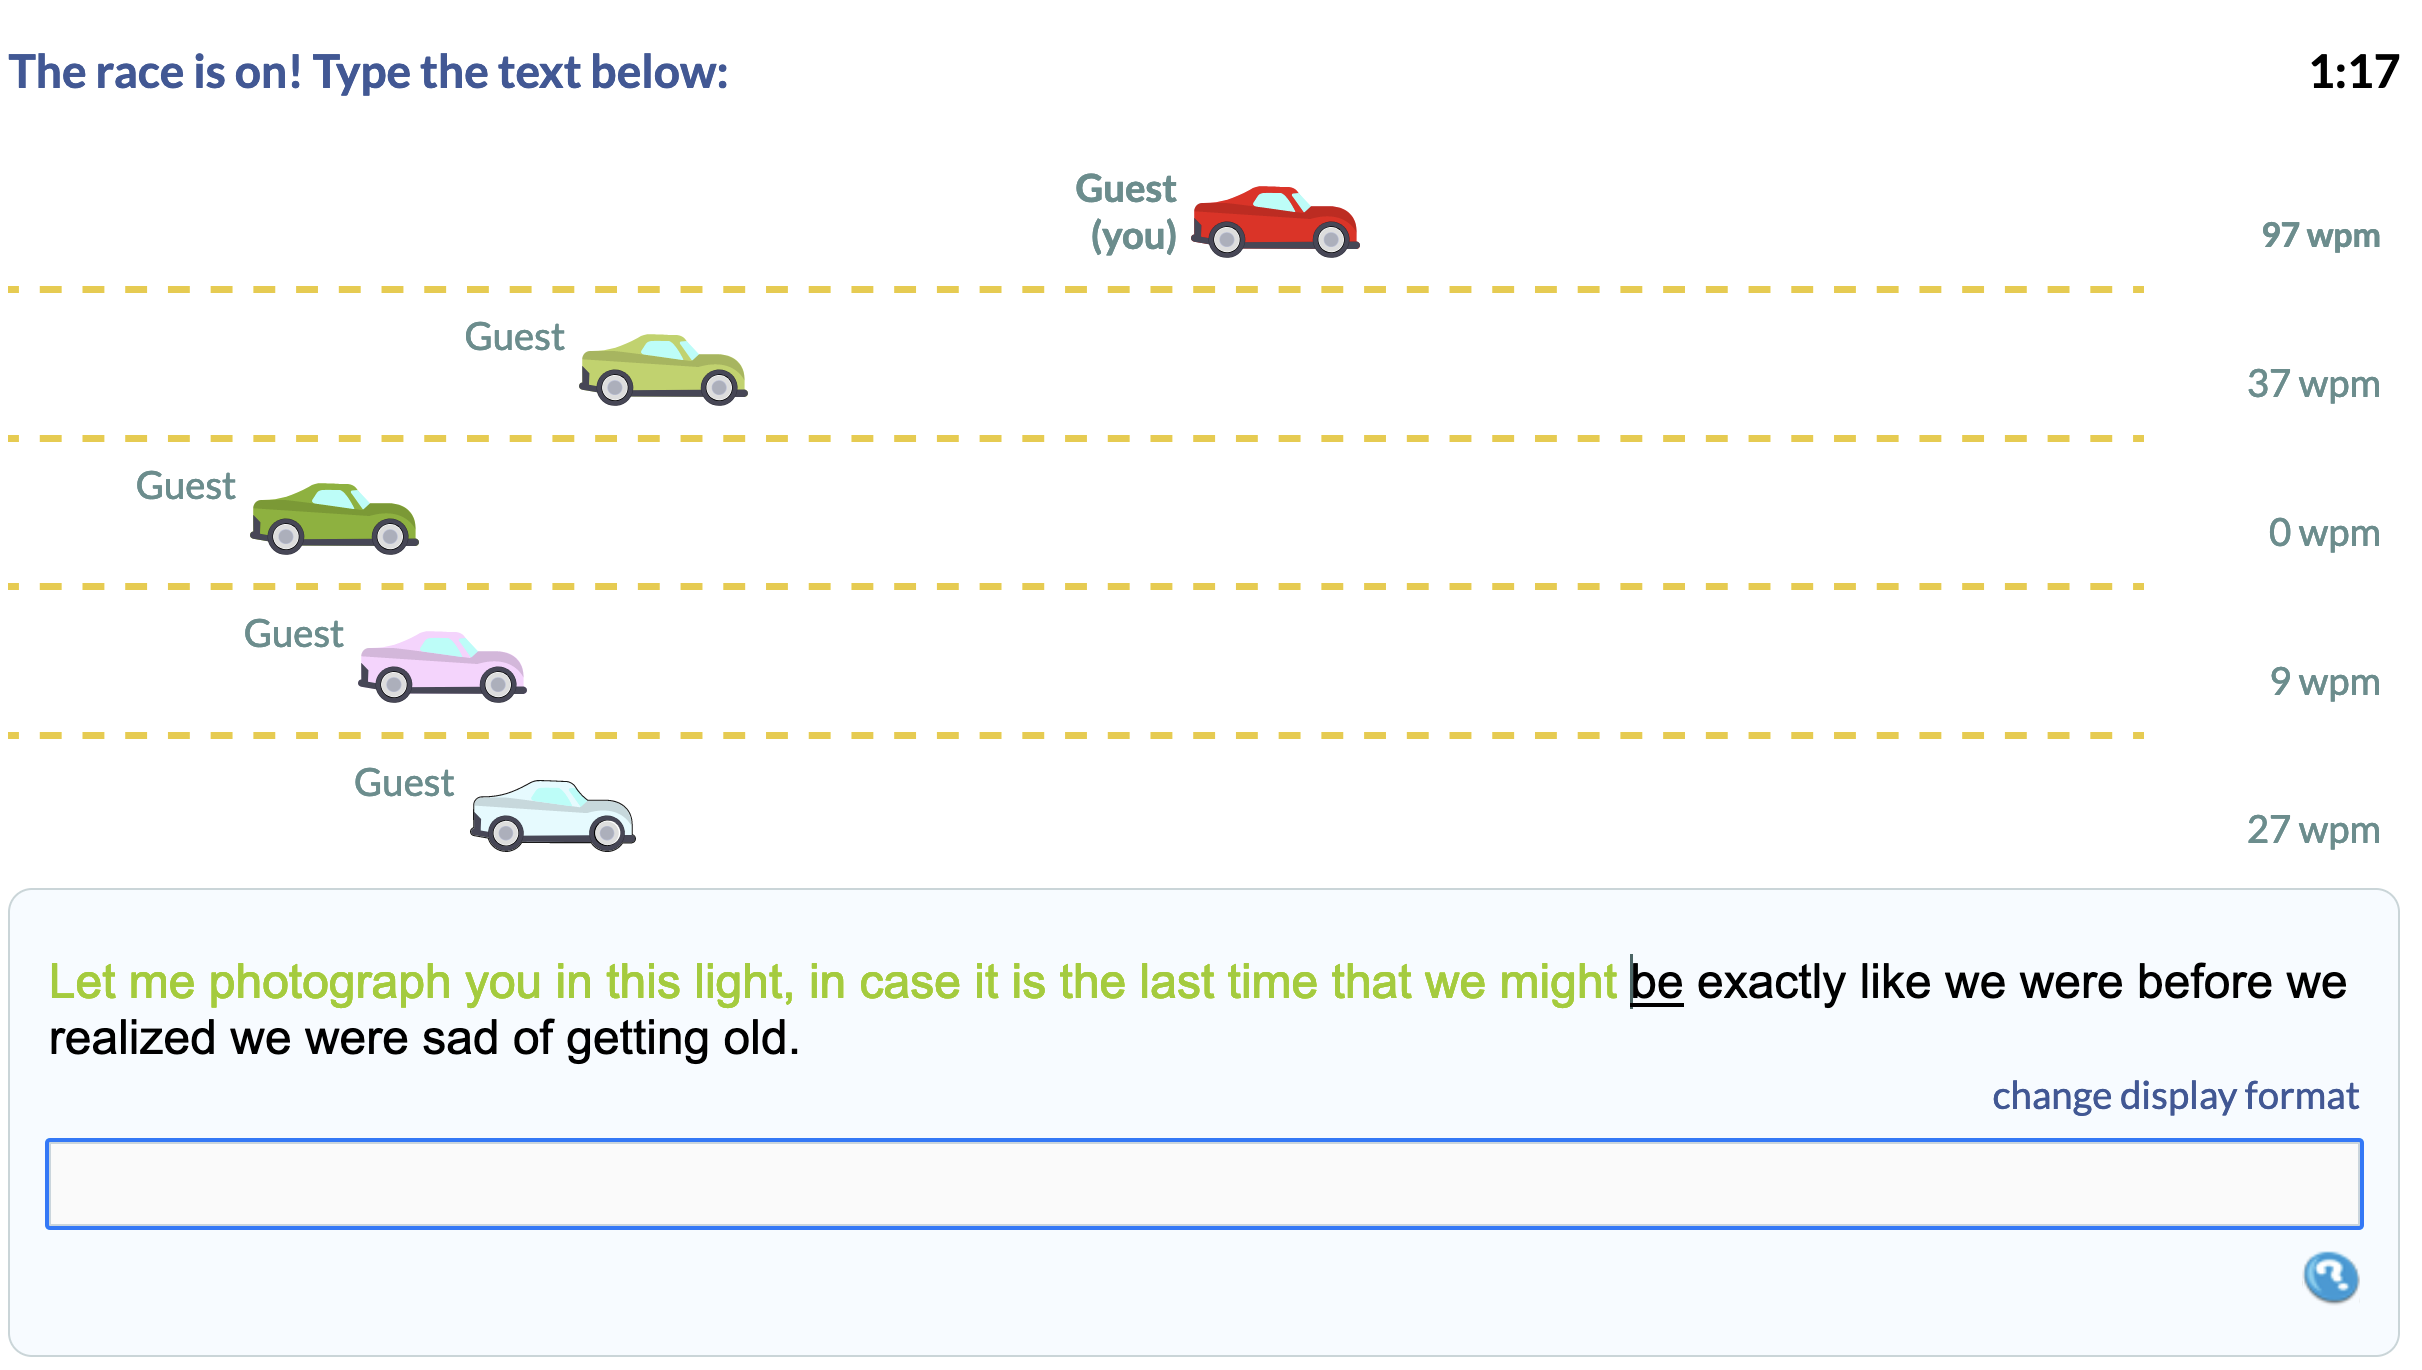
\includegraphics[width=\textwidth]{typeracer.png}
	\caption{A screenshot of a typing competition on the website \textit{TypeRacer}}
\end{figure}

Your score at the end of the race is a measurement of your average typing speed throughout the text. Typing speed is measured in the units ``words per minute'' (``WPM'' for short), where each ``word'' is defined as five characters, including spaces.

However, not all texts are created equal. Some texts are harder to type than others, whether it's from having longer words, frequent capital letters, etc.

\begin{figure}[H]
	\caption{Two different possible texts in TypeRacer. On the left, an easy text, and on the right, a more difficult text.}
	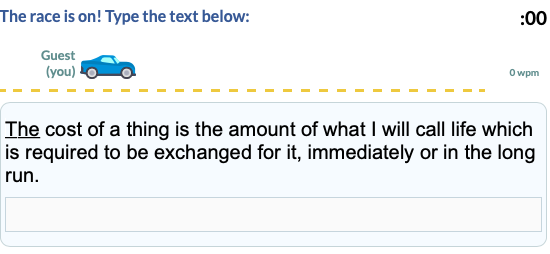
\includegraphics[width=0.5\textwidth]{easy-text.png}
	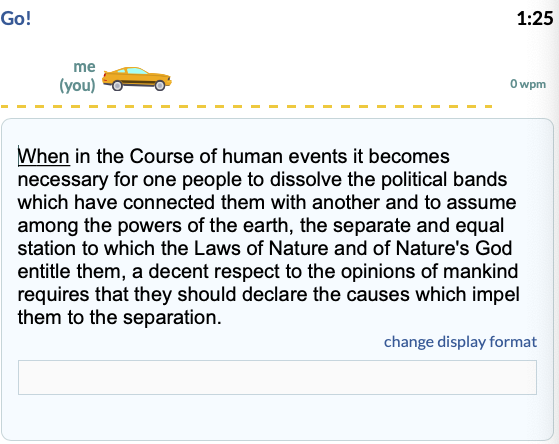
\includegraphics[width=0.5\textwidth]{hard-text.png}
\end{figure}

Currently, the way TypeRacer determines the difficulty of a text is through data collected from random players typing the text. If, on average, the players' speed on the text is lower than their average speed overall on other texts, then the text is classified as more difficult. If the players' speed on the text is greater than their overall speed, then the text is classified as easier to type.

Unfortunately, this approach of measuring text difficulty is biased towards users of the QWERTY keyboard layout, the most popular keyboard layout. In fact, I use an alternative keyboard layout called Programmer Dvorak (an image can be found in Figure 12 in the Appendix). Thus, a text containing words that may be difficult for QWERTY users to type (e.g. \texttt{minimum}) might be easier for me because my keyboard keys are arranged differently.

Thus, my goal in this exploration is to create a program that takes a certain text as input and outputs a prediction of how fast I would type the text. This program would analyze various characteristics of the text and correlate them with my typing speed by using my performance on past texts with similar characteristics. This program will use machine learning, which involves the use of algorithms and statistical models to analyze and detect patterns in data.

\section*{Gathering Data}

In order to create a machine learning algorithm that predicts how fast I can type a certain text, I need to collect a large amount of data that includes various texts and the speed at which I type them. Luckily, I've been active on TypeRacer for over 5 years now, and over these 5 years I've typed over 8000 texts on my account.

I created a program that automatically scrapes the race data from each of the 8000+ texts I've typed. I decided that for the scope of this exploration, I will only be using words that I've typed with 100\% accuracy (in other words, without making any mracesistakes). This is because accuracy is a fairly random measurement: just because I typed a word inaccurately once doesn't mean that the word is necessarily harder to type—it might have just been bad luck. After filtered out all the words that I didn't type perfectly, I was left with 20454 unique words to analyze.

\section*{Analyzing Data}

To take into consideration the gradual increase in my typing speed over time, the typing speed of a word should be measured relative to my average speed at the time. Thus, instead of using an absolute WPM measurement to measure a word's difficulty (since my average WPM changes over time), I've instead use a measurement of WPM ratio that compares the speed in WPM at which I typed the word at with my average monthly WPM at the time of typing the word:
\begin{align*}
	\text{WPM Ratio} & = \frac{\text{speed at which word was typed (in WPM)}}{\text{average monthly WPM at the time of typing the word}}
\end{align*}

After analyzing the data, I noticed some outliers in the data set. Occasionally, I take a short breather in the middle of a typing race if I'm making too many mistakes, and this is reflected in some of the data as it results in abnormally low speeds for some words. To counter this problem, I decided to take the median of the WPM ratios whenever there are multiple WPM ratios for a single word from multiple texts. I decided to use the median instead of the mean as the median wouldn't be as adversely affected by extreme data compared to the mean.

\section*{Predicting Typing Speed}

The WPM Ratio of a word depends on various features of the word, such as the length of the word and the amount of capital letters in the word.

For example, if the typing speed of a word was only linearly proportional to its length, then our predictive function might look like the following:
\begin{align*}
	\text{WPM Ratio} = w_{\text{word length}} \times (\text{word length}) + \text{Bias}
\end{align*}

This equation resembles the typical linear equation $y = mx + b$, where $w_{\text{word length}}$ represents the slope, or in other words, the amount that the WPM Ratio increases or decreases by when the word length is increased by 1.

However, when we plot a scatterplot of word length against WPM Ratio for our 20454, we obtain the following graph:

\begin{figure}[H]
	\caption{A graph of word length vs. WPM Ratio; each blue point represents a unique word collected from my TypeRacer typing data.}
	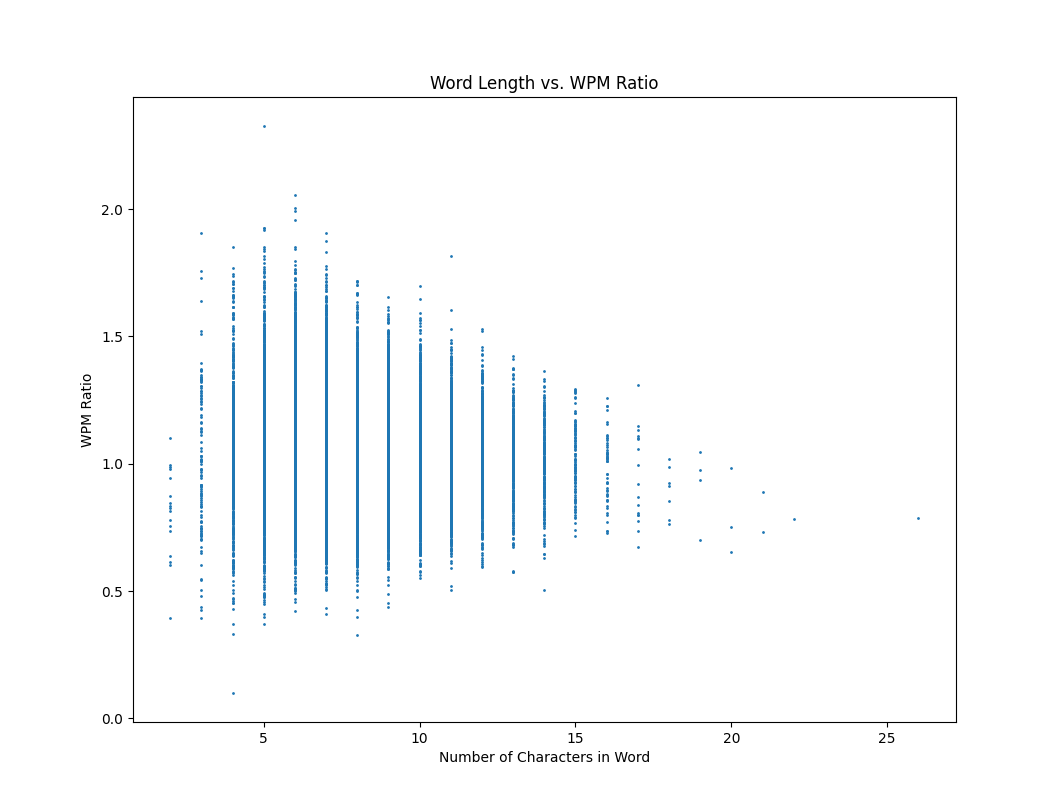
\includegraphics[width=\linewidth]{word-length-vs-wpm.png}
\end{figure}

The graph indicates that longer words typically have lower WPM Ratios, but the WPM ratios for shorter words varies significantly. If we sample some short words that have a WPM ratio lower than 0.5, we can understand why this is the case:


\begin{table}[H]
	\caption{Examples of words that are short but have low WPM ratios (i.e. hard to type).}
	\py{get_table()}
\end{table}

Even though these words are short, they contain capital letters and keys that need you to press the Shift key to type (\code{"} and \code{?}). This makes the word substantially slower to type, and isn't accounted for in Equation 1, which only considers the length of the word.

Thus, our WPM Ratio prediction function must take into account various features of the word that would affect typing speed. Some features, like the number of capital letters, will influence the word's typing speed more compared to other features, like whether the word starts with a vowel or a consonant.

To account for the different influences of different features, we need to assign a different weight to each of them in our equation, which gives us an equation similar to the following:
\begin{align*}
	\text{WPM Ratio} = w_1 \times (\text{Feature 1}) + w_2 \times (\text{Feature 2}) + \dots + \text{Bias}
\end{align*}

For example, if the only two features that influence the difficulty of a are the length of the word and the number of capital letters in the word, then the equation becomes:
\begin{align*}
	\text{WPM Ratio} = w_{\text{word length}} \times (\text{word length}) + w_{\text{\# of capital letters}} \times (\text{\# of capital letters}) + \text{Bias}
\end{align*}

In this equation, $w_{\text{word length}}$ isn't necessarily the same as $w_{\text{capital letters}}$. For example, if the magnitude of $w_{\text{word length}}$ is greater than $w_{\text{capital letters}}$, it means that the length of a word has more influence on the WPM ratio compared to the number of capital letters in the word.

Let us define our prediction function $f$ as a function that takes in a word $\text{Word}_i$ as input and returns the sum of the weights for each feature multiplied with the feature values of $\text{Word}_i$. The output of $f$ is our predicted WPM ratio for a certain word. If $w_i$ represents the weight for feature $i$, $x_{f_i}$ represents the feature value for feature $f$ of word $i$, and $b$ represents the bias term, then our WPM ratio equation can be written as:
\begin{align*}
	f(\text{Word}_i) & = w_1{x_1}_i + w_2{x_2}_i + \dots + w_n{x_n}_i + b
	\\
	f(\text{Word}_i) & = \Big(\sum_{f=1}^{n} w_f{x_f}_i\Big) + b
\end{align*}

To create an accurate prediction function, we need to find optimal values of $w_f$ that will give us predicted WPM ratios that are as close as possible to actual WPM ratios from our data. To find optimal values of $w_f$, we need to use a cost function that gives us a measure of how accurate our current values for $w_f$ are.

\subsection*{The Cost Function}

The cost function will give us a way to measure how accurate our prediction function $f$ is, and more importantly, how we can adjust the weights $w_f$ in our prediction function in order to reduce the cost.

One popular cost function used in machine learning is the MSE (Mean Squared Error). The MSE function defines the cost as the squares of the differences between the actual data ($y_i$) and the predicted data ($f(\text{Word}_i)$):
\begin{align*}
	C(f) & = \frac{1}{N}\big[(y_1 - f(\text{Word}_1))^2 + (y_2 - f(\text{Word}_2))^2 + \dots + (y_n - f(\text{Word}_n))^2]
	\\
	C(f) & = \frac{1}{N} \sum_{i=1}^{n} (y_i - f(\text{Word}_i))^2
\end{align*}

To visualize this cost function, I've plotted the below data for a small set of words that have a clear correlation between word length and WPM Ratio:


\begin{table}[H]
	\caption{The word length and WPM ratio for a small selection of words.}
	\noindent\begin{tabularx}{\linewidth}{|X|X|X|}
		\hline
		Word        &
		Word Length &
		WPM Ratio

		\py{get_table_row(0)}
		\py{get_table_row(1)}
		\py{get_table_row(2)}
		\py{get_table_row(3)}
		\py{get_table_row(4)}
		\py{get_table_row(5)}

		\\\hline
	\end{tabularx}
\end{table}

For a linear prediction function $f(\text{Word}_i) = w_1x_1 + b$, the cost function can be represented graphically as the sum of the squared lengths of the red lines in the graph below:

\begin{figure}[H]
	\centering
	\caption{A graph of the values in Table 2 with a suboptimal line of best fit. The red dots represent the actual data points and the red lines between these data points and the suboptimal line of best fit represent the cost. The goal of our function is to minimize the sum of the squared lengths of these red lines.}
	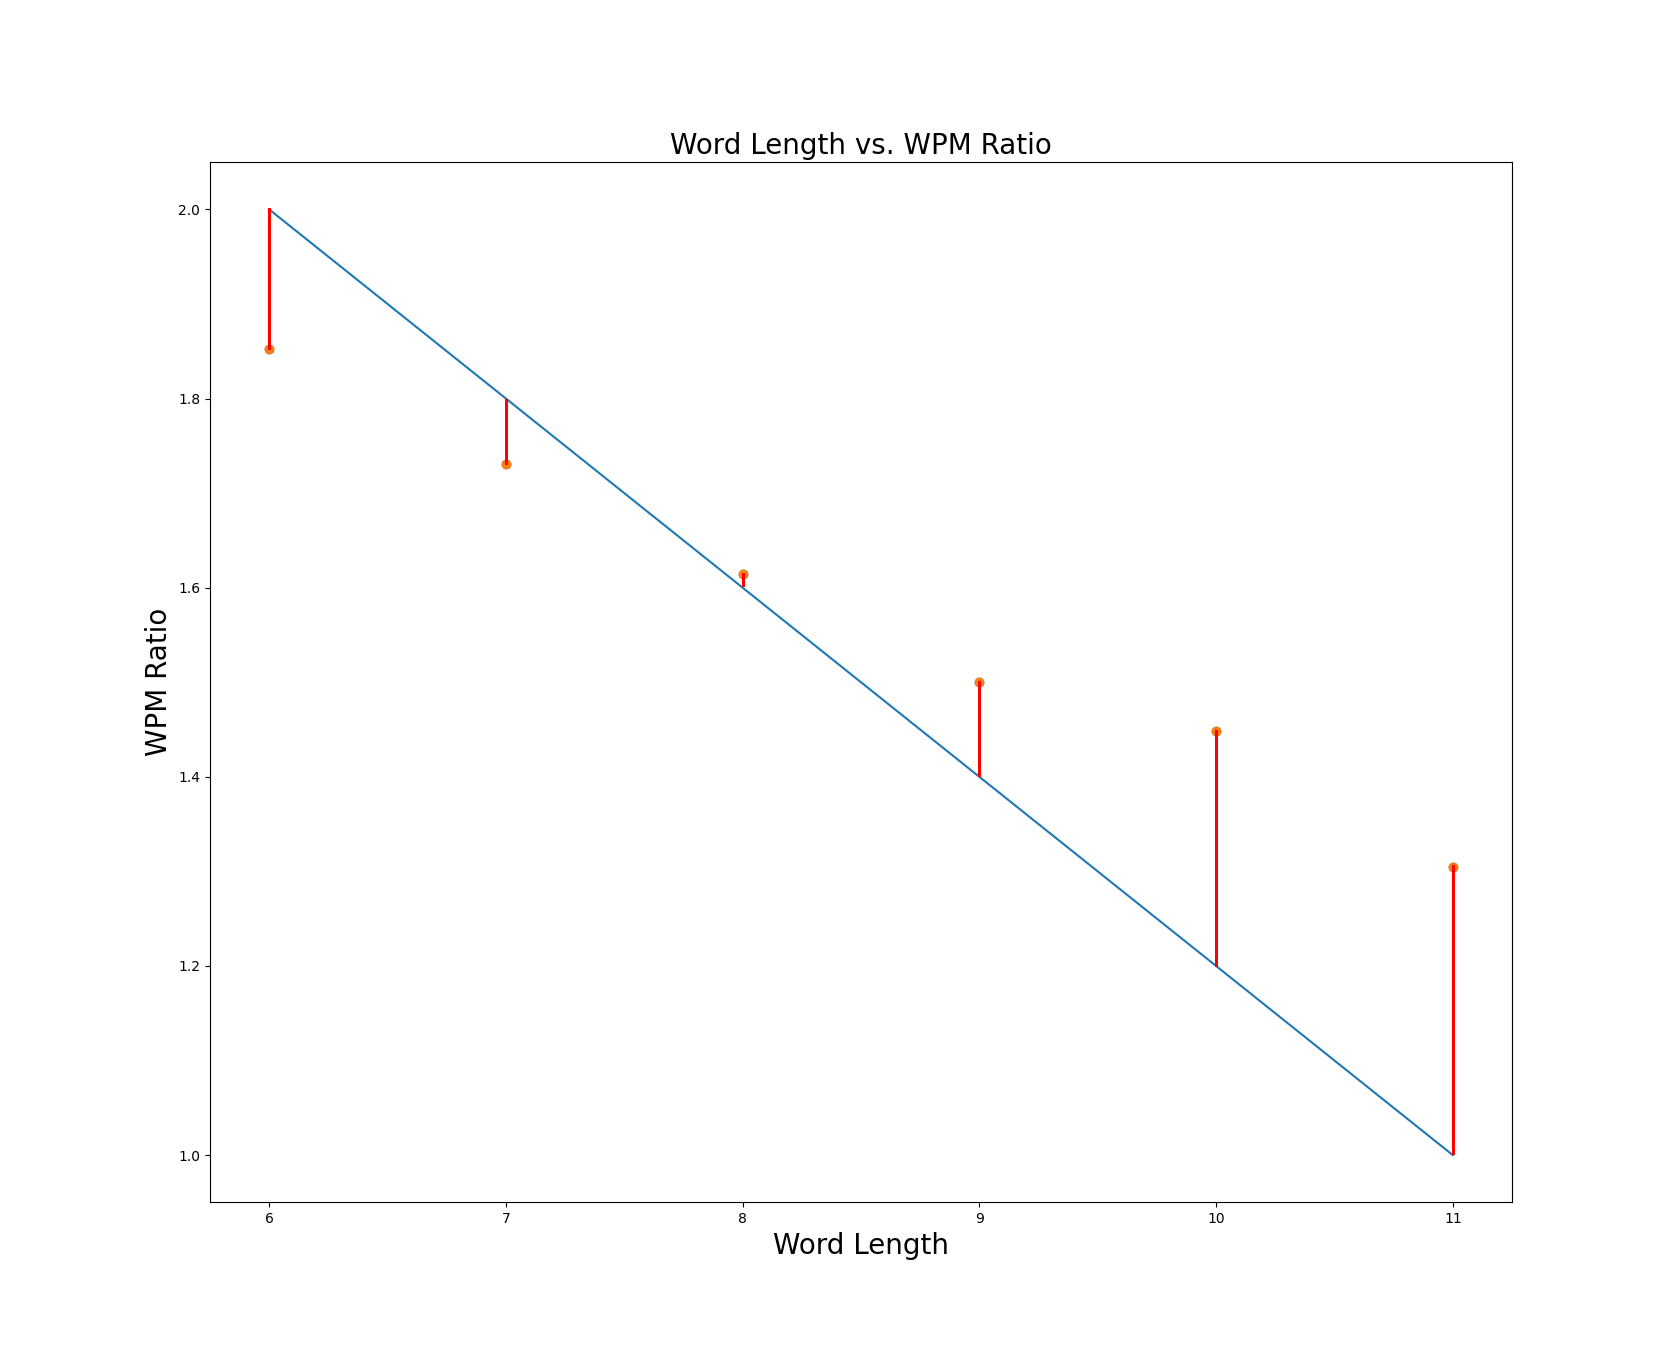
\includegraphics[width=\linewidth]{cost-visualization.png}
\end{figure}

The goal of our machine learning algorithm is to minimize this cost function: to find a set of weights for our prediction function $f$ such that $C(f)$ is as low as possible. A popular method for minimizing cost is by using gradient descent.

\subsection*{Gradient Descent}

Gradient descent involves using the derivative(s) of a function to find a function's local minimum. In our case, we need to find the local minimum of our cost function, $C$.

Let's consider the case where our prediction function $f$ is linearly correlated with only one weight, the text length. If we let $x_i$ represent the ``text length of word $i$'', our prediction function would look like the following:
\begin{align*}
	f(\text{Word}_i) = w_1x_i + b
\end{align*}

For this definition of $f$, our cost function would look like the following:
\begin{align*}
	C(w_1, b) & = \frac{1}{N} \sum_{i=1}^{n} (y_i - f(\text{Word}_i))^2
	\\
	C(w_1, b) & = \frac{1}{N} \sum_{i=1}^{n} (y_i - w_1x_i - b)^2
\end{align*}

To visualize this cost function, we can use a 3D graph where the x-axis correlates with various values of $w_1$, the y-axis correlates with various values of $b$, and the z-axis represents the cost (the value of $C(w_1, b)$). Using the values from Table 2 for our values of $x_i$ and $y_i$, a visual representation of our cost function would look like the following graph:
\begin{figure}[H]
	\centering
	\caption{A 3D visualization of our cost function plotted with GeoGebra using the equation $\py{get_geogebra_equation()}$. The red x-axis represents various values for $w_1$, the green y-axis represents various values for $b$, and the blue z-axis represents the cost $C(w_1, b)$.}
	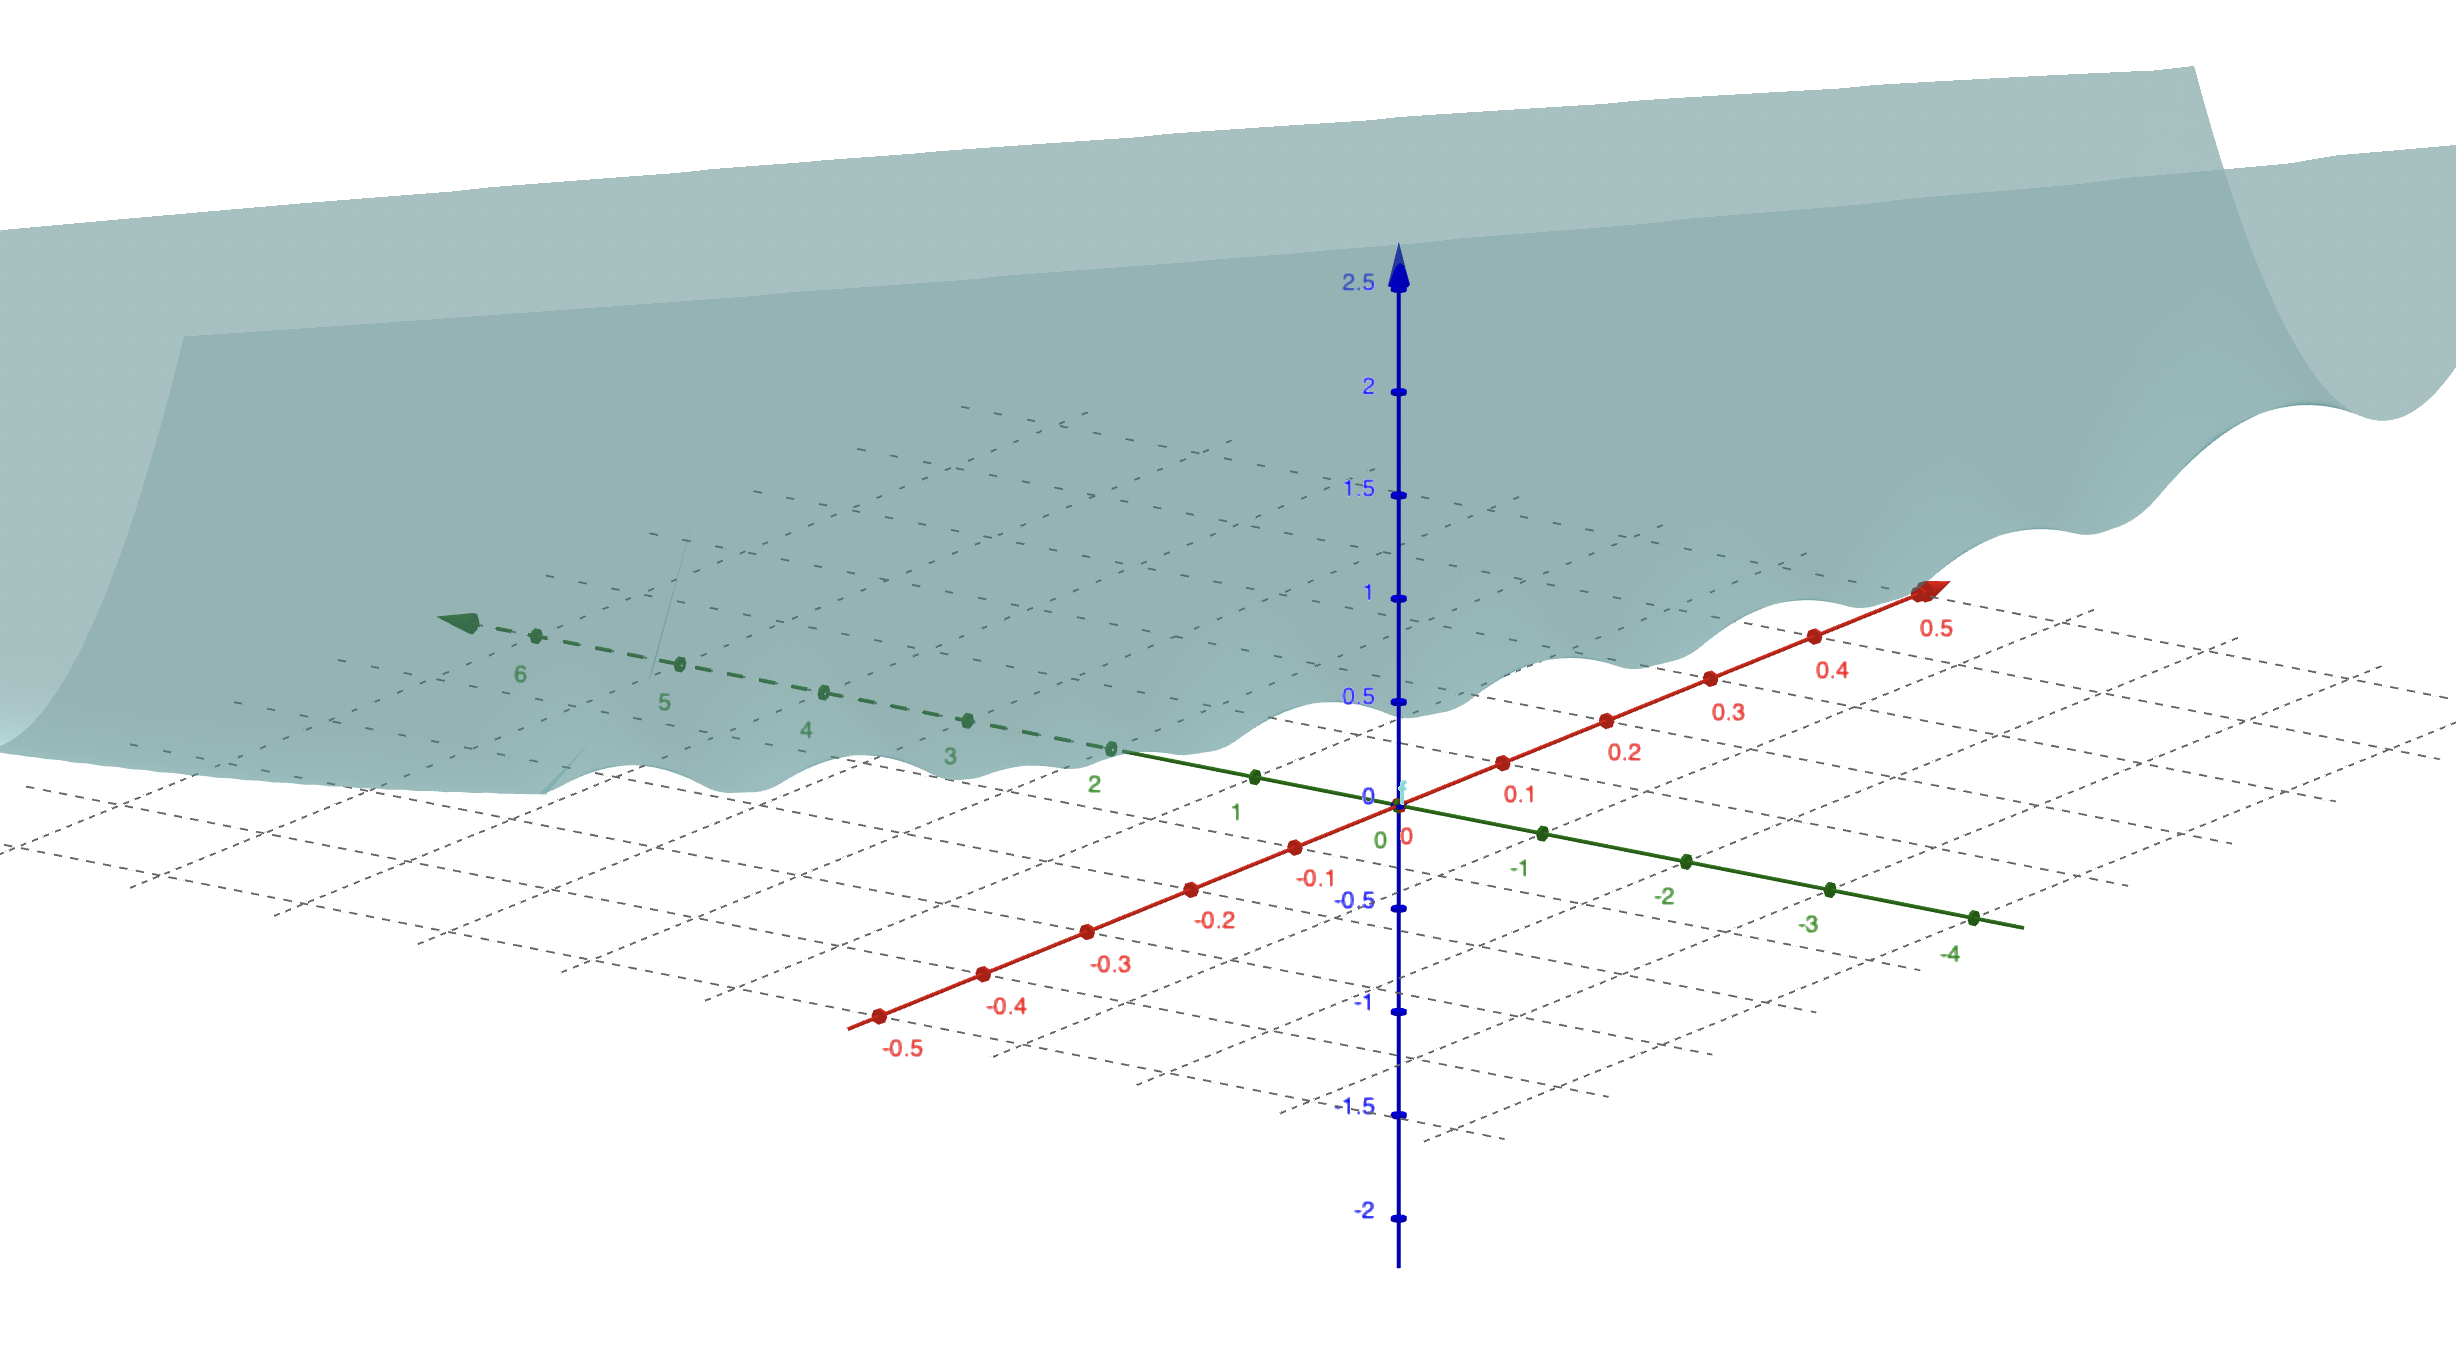
\includegraphics[width=\linewidth]{3d-plot.png}
\end{figure}

The goal of our machine learning algorithm is to find the minimum on the graph of $C(w_1, b)$. To find the minimum, we need to use the derivatives of $C(w_1, b)$. Since our cost function has more than one variable, $w_1$ and $b$, we need to use partial derivatives.

\subsection*{Partial Derivatives}

For a function that takes multiple variables, the gradient of the function is a vector where the $i$th value in the vector is the partial derivative of our function with respect to variable $i$. For our cost function $C(w_1, b)$, this means that the gradient, $\nabla Q$, is equal to:
\begin{align*}
	\nabla Q = \Big(\frac{dC}{dw_1}, \frac{dC}{db}\Big)
\end{align*}

When calculating each partial derivative, the other input variables for the function are treated as constants. For example, when calculating $\frac{dC}{dw_1}$, the bias term $b$ is treated as a constant:
\begin{align*}
	C(w_1, b)       & = \frac{1}{N} \sum_{i=1}^{n} (y_i - w_1x_i - b)^2
	\\
	\frac{dC}{dw_1} & = \frac{1}{N} \sum_{i=1}^{n} 2(y_i - w_1x_i - b) \times -x_i
	\\
	\frac{dC}{dw_1} & = -\frac{2}{N} \sum_{i=1}^{n} (y_i - w_1x_i - b) \times x_i
\end{align*}

Likewise, when calculating $\frac{dC}{db}$, the weight $w_1$ is treated as a constant:
\begin{align*}
	C(w_1, b)     & = \frac{1}{N} \sum_{i=1}^{n} (y_i - w_1x_i - b)^2
	\\
	\frac{dC}{db} & = \frac{1}{N} \sum_{i=1}^{n} 2(y_i - w_1x_i - b) \times -1
	\\
	\frac{dC}{db} & = -\frac{2}{N} \sum_{i=1}^{n} (y_i - w_1x_i - b)
\end{align*}

Thus, the gradient $\nabla Q$ of our cost function is equal to:
\begin{align*}
	\nabla Q = \Big(
	 &
	-\frac{2}{N} \sum_{i=1}^{n} (y_i - w_1x_i - b) \times x_i,
	\\
	 & -\frac{2}{N} \sum_{i=1}^{n} (y_i - w_1x_i - b)
	\Big)
\end{align*}

% Partial Derivative Example Calculation

Each partial derivative with respect to a variable tells us how the cost function would change if the variable changed. For example, if $w_1 = \py{weight}$, the partial derivative $\frac{dC}{dw_1}$ is equal to:
\begin{align*}
	\frac{dC}{dw_1} & = -\frac{2}{N} \sum_{i=1}^{n} (y_i - (\py{weight})x_i - (\py{bias})) \times x_i
	\\
	\frac{dC}{dw_1} & =
	\begin{aligned}[t]
		-\frac{2}{\py{len(x_values)}}
		\Big( & \py{get_expanded_summation()}\Big)
	\end{aligned}
	\\
	\frac{dC}{dw_1} & = \py{cost_derivative_str}
\end{align*}

Because the value of $\frac{dC}{dw_1}$ is positive, it indicates that increasing $w_1$ and keeping $b$ constant would increase the value of our cost function $C(w_1, b)$. This means that our current value of $w_1$ is greater than the optimal value of $w_1$, and to minimize our cost function, we should decrease $w_1$.


This process is repeated for each partial derivative. For example, if our current bias value is $b = \py{bias}$, the partial derivative $\frac{dC}{db}$ is equal to:
\begin{align*}
	\frac{dC}{db} & = -\frac{2}{N} \sum_{i=1}^{n} (y_i - (\py{weight})x_i - (\py{bias}))
	\\
	\frac{dC}{db} & =
	\begin{aligned}[t]
		-\frac{2}{\py{len(x_values)}}
		\Big( & \py{get_expanded_summation_bias()}\Big)
	\end{aligned}
	\\
	\frac{dC}{db} & = \py{cost_derivative_bias_str}
\end{align*}

In this case, since $\frac{dC}{db}$ is negative when $b = \py{bias}$, it indicates that increasing $b$ will decrease the cost. This means that our current value of $b$ is below the optimal value of $b$, and that we should increase it to minimize the cost.

The hyperparameter that determines how much we increase/decrease each variable by is called the learning rate, $\eta$. To find the new weight, $w_1'$, we add the current weight $w_1$ to the learning rate times the negative gradient. We use the negative gradient so that when our gradient is positive, we decrease the variable to decrease our cost, and when our gradient is negative, we increase the variable to decrease our cost:
{
\setlength{\abovedisplayskip}{0pt}
\setlength{\belowdisplayskip}{0pt}
\begin{center}
	\noindent\begin{tabularx}{0.8\linewidth}{X X}
		\vbox{
			\begin{align*}
				w_1' & = w_1 + (-\frac{dC}{dw_1} \times \eta)
				\\
				w_1' & = w_1 - \frac{dC}{dw_1} \times \eta
				\\
				w_1' & = \py{weight} - (\py{cost_derivative_str}) \times \eta
			\end{align*}
		}
		 &
		\vbox{
			\begin{align*}
				b' & = b + (-\frac{dC}{db} \times \eta)
				\\
				b' & = b - \frac{dC}{db} \times \eta
				\\
				b' & = \py{bias} - (\py{cost_derivative_bias_str}) \times \eta
			\end{align*}
		}
	\end{tabularx}
\end{center}
}
{
\setlength{\abovedisplayskip}{0pt}
\setlength{\belowdisplayskip}{0pt}
For example, if we set $\eta$ equal to \py{learning_rate}, then the new values for our weight and bias are:
\begin{center}
	\begin{tabularx}{0.8\linewidth}{X X}
		\vbox{
			\begin{align*}
				w_1' & = \py{weight} - (\py{cost_derivative_str}) \times \py{learning_rate}
				\\
				w_1' & = \py{weight} - (\py{f3f(cost_derivative * learning_rate)})
				\\
				w_1' & = \py{f3f(weight - cost_derivative * learning_rate)}
			\end{align*}
		} &
		\vbox{
			\begin{align*}
				b' & = \py{bias} - (\py{cost_derivative_bias_str}) \times \py{learning_rate}
				\\
				b' & = \py{bias} - (\py{f3f(cost_derivative_bias * learning_rate)})
				\\
				b' & = \py{f3f(bias - cost_derivative_bias * learning_rate)}
			\end{align*}
		}
	\end{tabularx}
\end{center}
}

One limitation with gradient descent is that it's possible for the machine learning model to converge at a local minimum for the cost function instead of arriving at the global minimum. However, in practice, the local minimum of complex cost functions are generally close to the global minimum, which is why gradient descent remains a popular method to minimizing the cost function in machine learning models.

However, how do we know what value of $\eta$ we should use? In other words, how much should increase or decrease $w_1$ by? If we increase/decrease the weight by too much, we could end up in a position of higher loss than we were before. If we move increase/decrease the weight too slowly, it will take a long time before we find the minimum:

\begin{figure}[H]
	\centering
	\caption{Increasing by too much would overshoot the local minimum; increasing by too little would take too long to reach the local minimum.}
	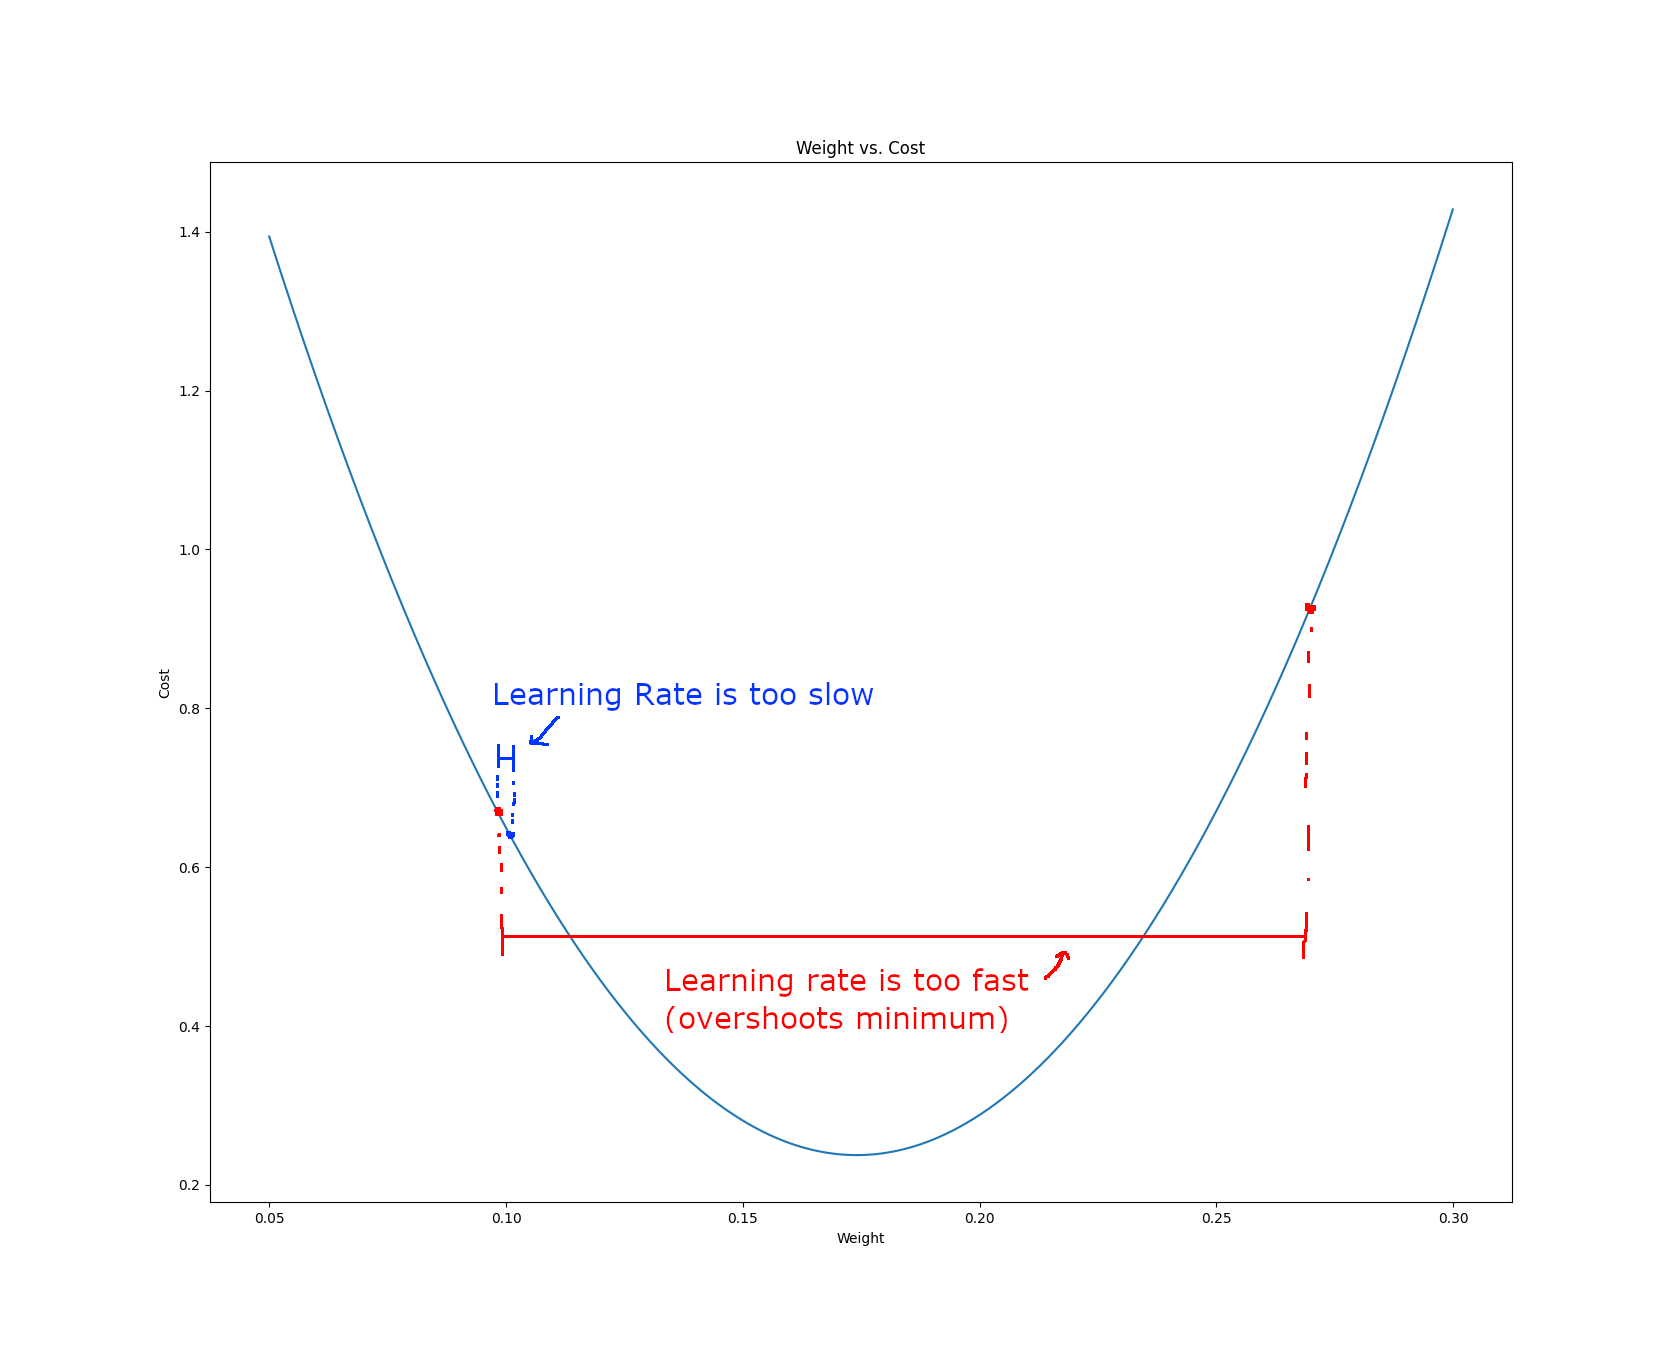
\includegraphics[width=\linewidth]{learning-rate.png}
\end{figure}

The optimal choice of $\eta$ will vary for different situations, but there are heuristics that can help. When the learning rate is too high, the cost function will increase infinitely, indicating that the learning rate should be decreased by an order of magnitude. In my case, I simply monitored the cost after each iteration and used trial-and-error to find an optimal learning rate.

I created a Python program to run the above calculations for the values in Table 2 until the difference between $C(w_1, b)$ and $C(w_1', b')$ was less than $10^{-9}$, indicating that the machine learning model had converged. I set the learning rate $\eta$ to 0.01, and after 8341 iterations, the program outputted the following values for $w_1$ and $b$ (to 9 decimal places):
\begin{align}
	w_1 & = -0.105086863 \\
	b   & = 2.472476099
\end{align}

If we substitute these values for $w_1$ and $b$ into our prediction function $f$ and plot our function on a graph alongside the data from Table 2, we obtain the following graph:
\begin{figure}[H]
	\centering
	\caption{A graph of our prediction function $f$ using the values from Equations 1 and 2.}
	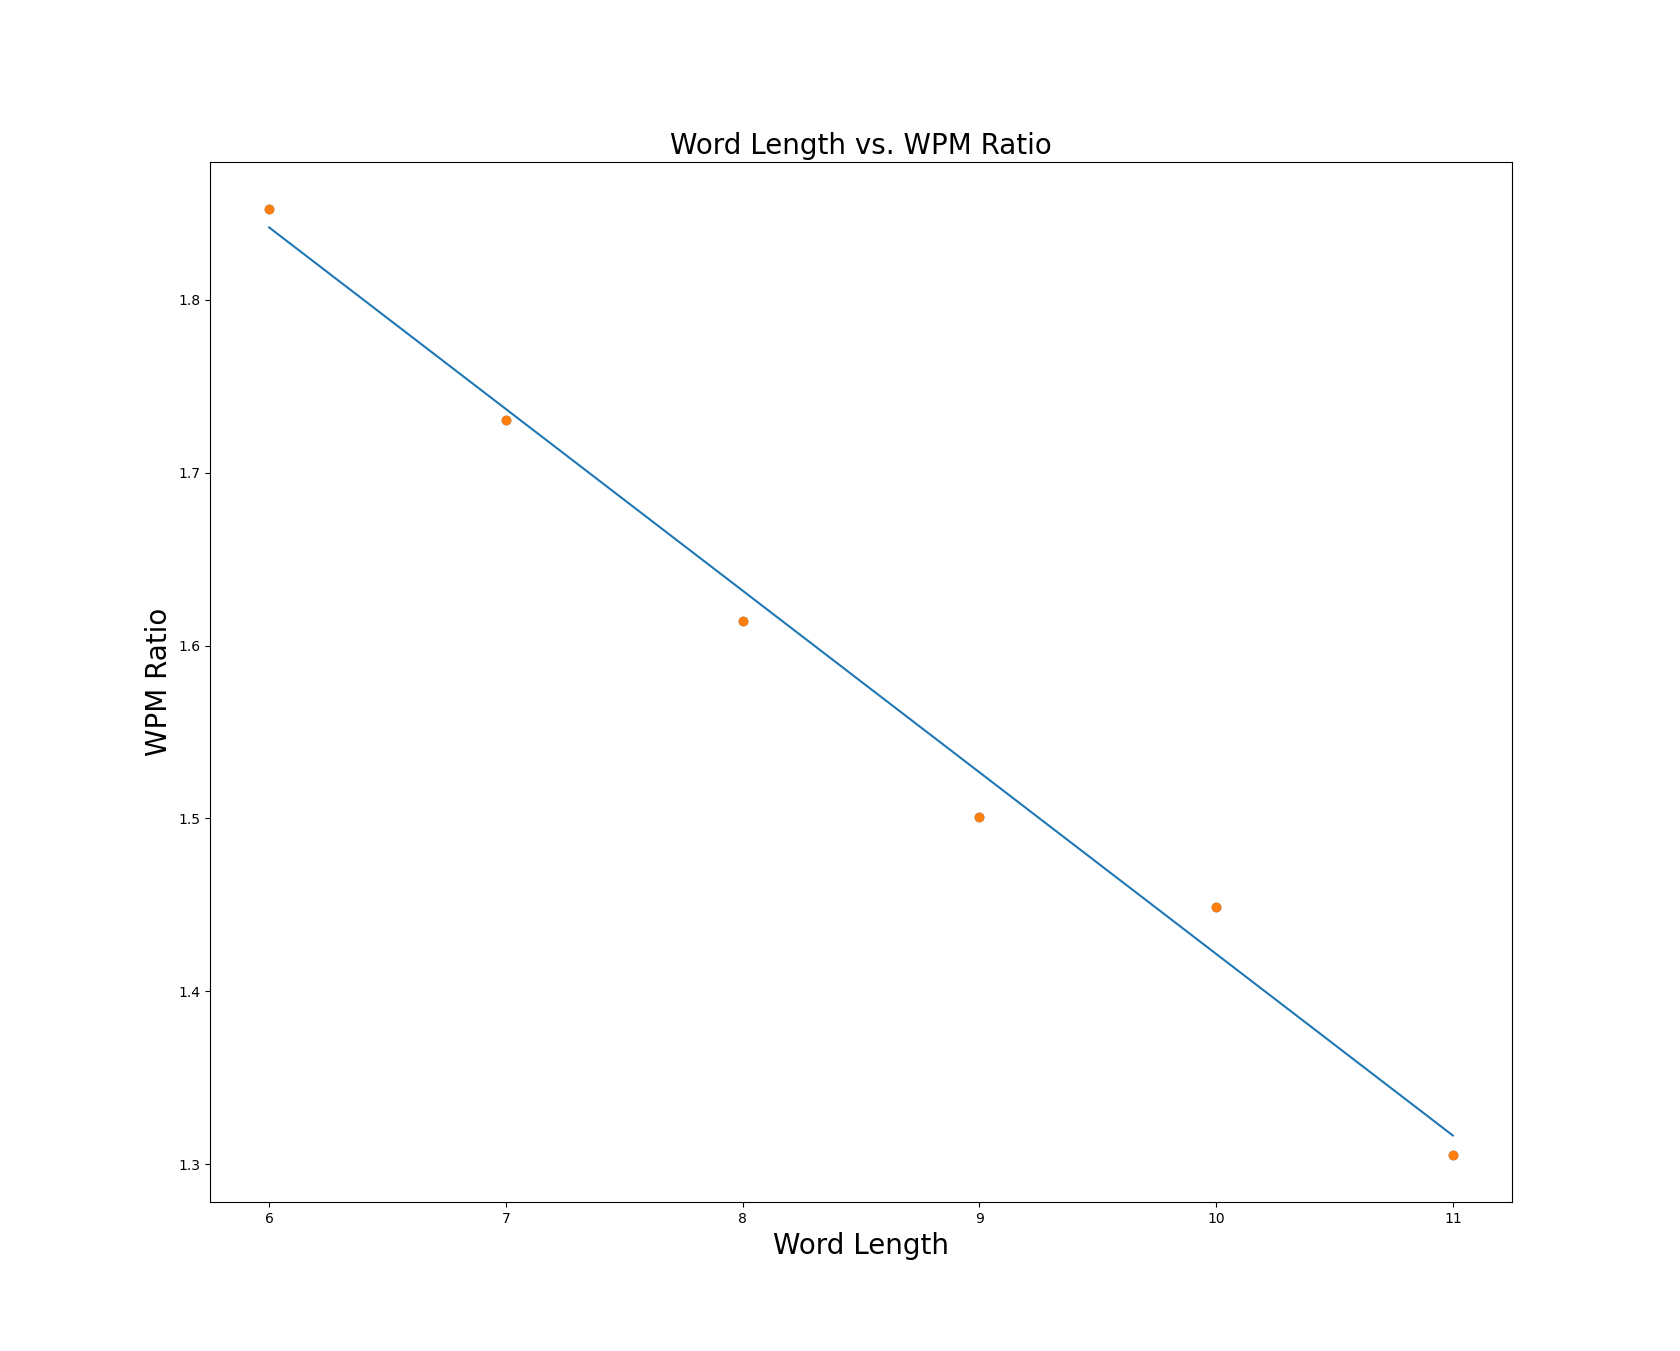
\includegraphics[width=\textwidth]{word-length-vs-wpm-ratio.png}
\end{figure}

In my program, I've also tracked the value of the cost function $C(w_1, b)$ after each iteration. Plotting the cost against the iteration number gives us the following graph:
\begin{figure}[H]
	\centering
	\caption{A graph of iteration number versus cost when running the machine learning model with the values in Table 2. The cost initially decreases steeply, but overtime it decreases more slowly.}
	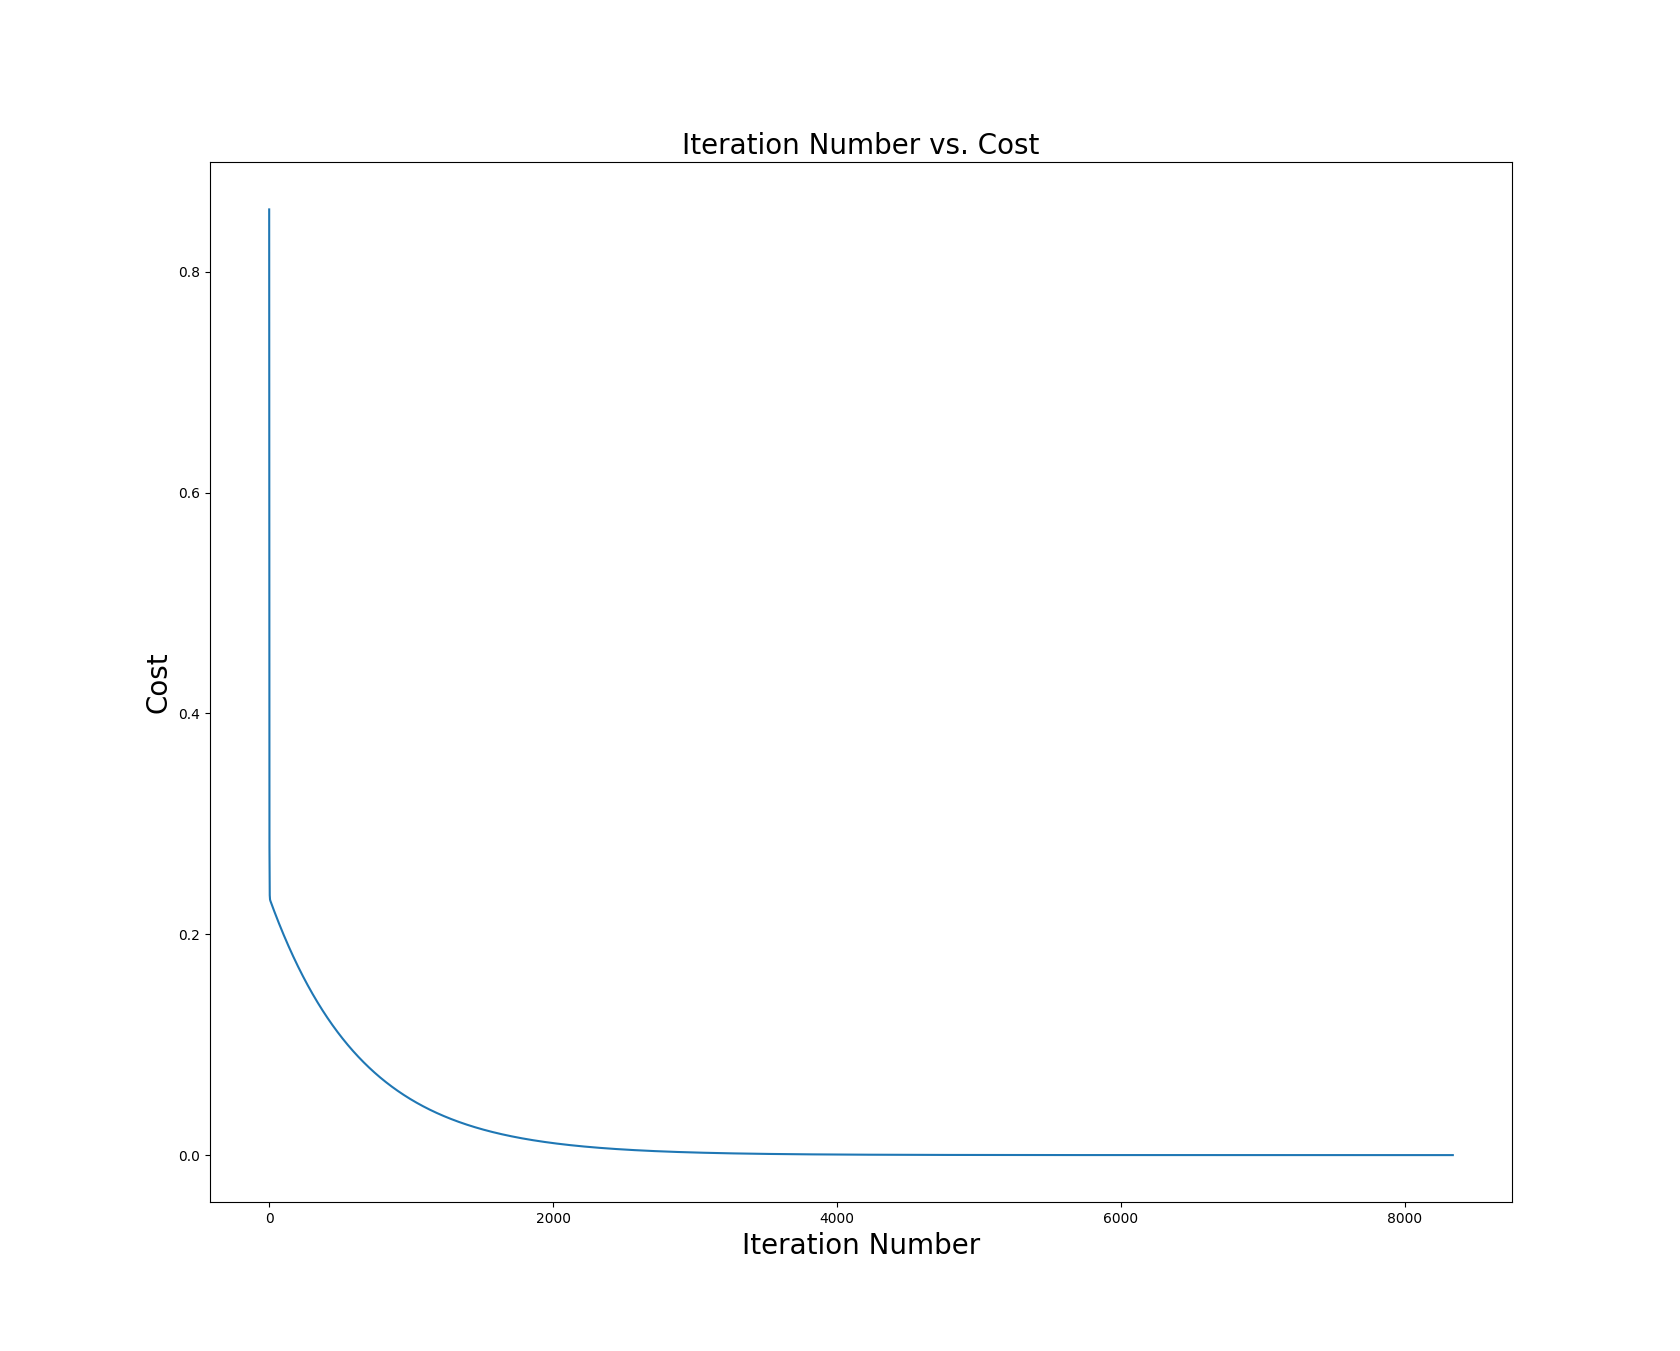
\includegraphics[width=\textwidth]{iteration-no-vs-cost.png}
\end{figure}

However, as indicated by the graph in Figure 3, the WPM ratio isn't just correlated with the word length. Thus, we need to apply our machine learning algorithms for a prediction function that takes into account more features in addition to the word length.

\subsection*{Analyzing More Features}

There are many characteristics of a word that can affect its WPM ratio. Below is a list of features that I will be analyzing and using to create an accurate prediction function for predicting the WPM ratio of a word:

\begin{itemize}
	\item The number of characters in the word (word length).
	\item The number of capital letters in the word.
	\item The number of times the same finger is used to type consecutive letters in the word. For example, the word ``mummy'' requires using the right index finger five times in a row on a QWERTY keyboard.
	\item The number of sets of ``double letters'' in the word. For example, the word ``sheep'' has 1 set of double letters, and the word ``bittersweet'' has 2 sets of double letters.
	\item The number of letters in the home row of the keyboard (on a QWERTY keyboard, this is the row with the letters ``asdf'').
	\item The number of letters typed with the left hand.
	\item The number of letters typed with the right hand.
	\item The number of letters that require pressing the Shift key to type.
	\item Whether the word is common (1 if the word is included within the top 1000 most common English words, and 0 otherwise).
\end{itemize}

I've created a program that extracts these features from every word. Table 3 contains three examples of words processed by my program and the value of each of these features for these words:


\begin{table}[H]
	\def\arraystretch{1.3}
	\caption{Three examples of features in words.  The following data might not match with the data expected from a QWERTY layout, and that's because when analyzing my typing data, I based it off the keyboard layout that I use—the Programmer Dvorak layout (refer to Figure 12 in the Appendix for more information).}
	\begin{tabularx}{\linewidth}{|
			p{70pt}|
			>{\RaggedRight}X|
			>{\RaggedRight}X|
			>{\RaggedRight}X|
			>{\RaggedRight}X|
			>{\RaggedRight}X|
			>{\RaggedRight}X|
		}
		\hline

		Word                               &
		\# of Characters                   &
		\# of Capitals                     &
		\# of Same-Finger Consecutive Keys &
		\# of Double Letters               &
		\# of Home Row Letters

		\py{get_table_1_row(word1)}
		\py{get_table_1_row(word2)}
		\py{get_table_1_row(word3)}
		\\\hline
	\end{tabularx}

	\vspace{2ex}

	\begin{tabularx}{\linewidth}{|
			p{70pt}|
			>{\RaggedRight}X|
			>{\RaggedRight}X|
			>{\RaggedRight}X|
			>{\RaggedRight}X|
			>{\RaggedRight}X|
			>{\RaggedRight}X|
			>{\RaggedRight}X|
		}
		\hline

		Word                          &
		\# of Left Hand Letters       &
		\# of Right Hand Letters      &
		\# of Letters Requiring Shift &
		Is word common?               &
		Median WPM

		\py{get_table_2_row(word1)}
		\py{get_table_2_row(word2)}
		\py{get_table_2_row(word3)}
		\\\hline
	\end{tabularx}
\end{table}

To incorporate all these features into our prediction function, we need to include more terms in our equation. If we define $w_f$ to represent the weight of feature $f$ and the value of feature $f$ of word $i$ as ${x_f}_i$, then our new prediction function would look like:
\begin{align*}
	f(\text{Word}_i) & = w_1{x_1}_i + w_2{x_2}_i + \dots + w_{9}{x_{9}}_i + b
	\\
	f(\text{Word}_i) & = \Big(\sum_{f=1}^{9} w_f{x_f}_i\Big) + b
\end{align*}

Our cost function would also change:
\begin{align*}
	C(f)                          & = \frac{1}{9} \sum_{i=1}^{9} (y_i - f(\text{Word}_i))^2
	\\
	C(w_1, w_2, \dots, w_{9}, b) & = \frac{1}{9} \sum_{i=1}^{n} (y_i - w_1{x_1}_i - w_2{x_2}_i - \dots - w_{9}{x_{9}} - b)
\end{align*}

The new gradient $\nabla Q$ for our cost function would now be:
\begin{align*}
	\nabla Q & = \Big(\frac{dC}{dw_1}, \frac{dC}{dw_2}, \dots, \frac{dC}{dw_{9}}, \frac{dC}{db}\Big)
	\\
	\nabla Q & =
	\begin{aligned}[t]
		\Big(
		 & -\frac{2}{9} \sum_{i=1}^{n} (y_i - w_1{x_1}_i - w_2{x_2}_i - \dots - w_{9}{x_{9}}_i - b) \times {x_1}_i,
		\\
		 & -\frac{2}{9} \sum_{i=1}^{n} (y_i - w_1{x_1}_i - w_2{x_2}_i - \dots - w_{9}{x_{9}}_i - b) \times {x_2}_i,
		\\
		 & \vdots
		\\
		 & -\frac{2}{9} \sum_{i=1}^{n} (y_i - w_1{x_1}_i - w_2{x_2}_i - \dots - w_{9}{x_{9}}_i - b) \times {x_{9}}_i,
		\\
		 & -\frac{2}{9} \sum_{i=1}^{n} (y_i - w_1{x_1}_i - w_2{x_2}_i - \dots - w_{9}{x_{9}}_i - b)
		\Big)
	\end{aligned}
\end{align*}

After each iteration, we need to update all 9 weights:
\begin{align*}
	w_1' & = w_1 - \frac{dC}{dw_1} \times \eta,
	\;
	w_2' = w_2 - \frac{dC}{dw_2} \times \eta,
	\;
	\dots,
	\;
	w_{9}' = w_{9} - \frac{dC}{dw_{9}} \times \eta
	\\
	b'   & = b - \frac{dC}{db} \times \eta
\end{align*}

The above equations involve many separate variables, which makes implementing the algorithm with code more difficult. Luckily, we can simplify the above equations using vectors.

Let us denote $\vec{X_i}$ as a vector whose length is 9, which is equal to the number of features in each word. $\vec{X_i}$ contains all the values of the features of $\text{Word}_i$. Let us denote $\vec{W}$ as a vector also of length 9 containing all the weights for each feature. Using these vector definitions, we can use vectors to represent our prediction function:
\begin{align*}
	f(\text{Word}_i) & = \Big(\sum_{f=1}^{9} w_f{x_f}_i\Big) + b
	\\
	f(\text{Word}_i) & = \vec{X_i} \cdot \vec{W} + b
\end{align*}

To further simplify this equation, we can define $\vec{X}_i$ as a vector of length 10 instead—1 greater than the number of features in each word. In addition to containing all the values of the features of $\text{Word}_i$, we add a constant 1 to the end of $\vec{X}_i$:
\begin{align*}
	\vec{X}_i = ({x_1}_i, {x_2}_i, \dots, {x_{9}}_i, 1)
\end{align*}

This way, if we redefined $\vec{W}$ to be a vector of length 10 which contains all the weights \textit{and} the bias term:
\begin{align*}
	\vec{W} = (w_1, w_2, \dots, w_{9}, b)
\end{align*}

Our prediction function could then be written as:
\begin{align*}
	f(\text{Word}_i) = \vec{X_i} \cdot \vec{W}
\end{align*}

Since this would be equal to:
\begin{align*}
	f(\text{Word}_i) & = w_1{x_i}_1 + w_2{x_i}_2 + \dots + w_{9}{x_i}_{9} + (1)(b)
	\\
	f(\text{Word}_i) & = \Big(\sum_{f=1}^{9} w_f{x_f}_i\Big) + b
\end{align*}

Which is equal to our initial prediction function.

\bigskip

Using vectors, we can also simplify our cost function:
\begin{align*}
	C(f)       & = \frac{1}{9} \sum_{i=1}^{9} (y_i - f(\text{Word}_i))^2
	\\
	C(\vec{W}) & = \frac{1}{9} \sum_{i=1}^{9} (y_i - \vec{W} \cdot \vec{X_i})^2
\end{align*}

And finally, we can simplify our gradient $\nabla Q$:
\begin{align*}
	\nabla Q & = \Big(\frac{dC}{dw_1}, \frac{dC}{dw_2}, \dots, \frac{dC}{dw_{9}}, \frac{dC}{db}\Big)
	\\
	\nabla Q & =
	\begin{aligned}[t]
		\Big(
		 & -\frac{2}{9} \sum_{i=1}^{n} (y_i - \vec{W} \cdot \vec{X_i}) \times {x_i}_1,
		\\
		 & -\frac{2}{9} \sum_{i=1}^{n} (y_i - \vec{W} \cdot \vec{X_i}) \times {x_i}_2,
		\\
		 & \vdots
		\\
		 & -\frac{2}{9} \sum_{i=1}^{n} (y_i - \vec{W} \cdot \vec{X_i}) \times {x_i}_{9},
		\\
		 & -\frac{2}{9} \sum_{i=1}^{n} (y_i - \vec{W} \cdot \vec{X_i})
		\Big)
	\end{aligned}
\end{align*}

With vectors, updating the weights now becomes a simple one-liner:
\begin{align*}
	\vec{W}' = \vec{W} - \eta\nabla Q
\end{align*}

Not only do vectors allow us to represent our equations more succinctly, but they also make implementing them in code much easier.

\section*{Results}

Using the above vector equations, I've implemented a Python program that processes the features of all 20454 words and uses their actual WPM ratio as the values of $y_i$ to find the optimal set of weights that minimizes the cost function $C(\vec{W})$. I used a learning rate of 0.008 and trained my model over 100000 iterations, which took around 12 hours on my computer. After the program finished executing, it produced the following weights:
\begin{align*}
	w_{\text{\# of characters}}
	 & = \py{final_weights[0]}
	\\
	w_{\text{\# of capitals}}
	 & = \py{final_weights[1]}
	\\
	w_{\text{\# of same-finger consecutive letters}}
	 & = \py{final_weights[2]}
	\\
	w_{\text{\# of double letters}}
	 & = \py{final_weights[3]}
	\\
	w_{\text{\# of home row letters}}
	 & = \py{final_weights[4]}
	\\
	w_{\text{\# of left hand letters}}
	 & = \py{final_weights[5]}
	\\
	w_{\text{\# of right hand letters}}
	 & = \py{final_weights[6]}
	\\
	w_{\text{\# of letters requiring shift}}
	 & = \py{final_weights[7]}
	\\
	w_{\text{is word common}}
	 & =\py{final_weights[8]}
	\\
	b
	 & = \py{final_weights[9]}
\end{align*}

A negative weight indicates that the feature makes a text more difficult and a positive weight indicates that the feature makes a text easier. If a feature weight is larger, it indicates that the feature has more influence over the difficulty of a text. As expected, whenever a text has more characters, more capital letters, more same-finger consecutive letters, and more letters requiring the Shift key, it makes the text harder. Whenever the text is common or has more home row letters, it makes the text easier.

However, what I found interesting is that the number of double letters seems to make a text easier to type, which is contrary to intuition that typing the same letter twice would typically slow you down. I believe that the reason for this is because compared to other features of a text (e.g. capital letters), double letters are quicker to type, so my machine learning algorithm ended up correlating double letters to typing a word faster.

As expected, the cost vs. iteration graph shows the cost decreasing as more iterations are performed:
\begin{figure}[H]
	\caption{The graph of iteration number versus cost ($C(\vec{W})$) plotted on a logarithmic scale.}
	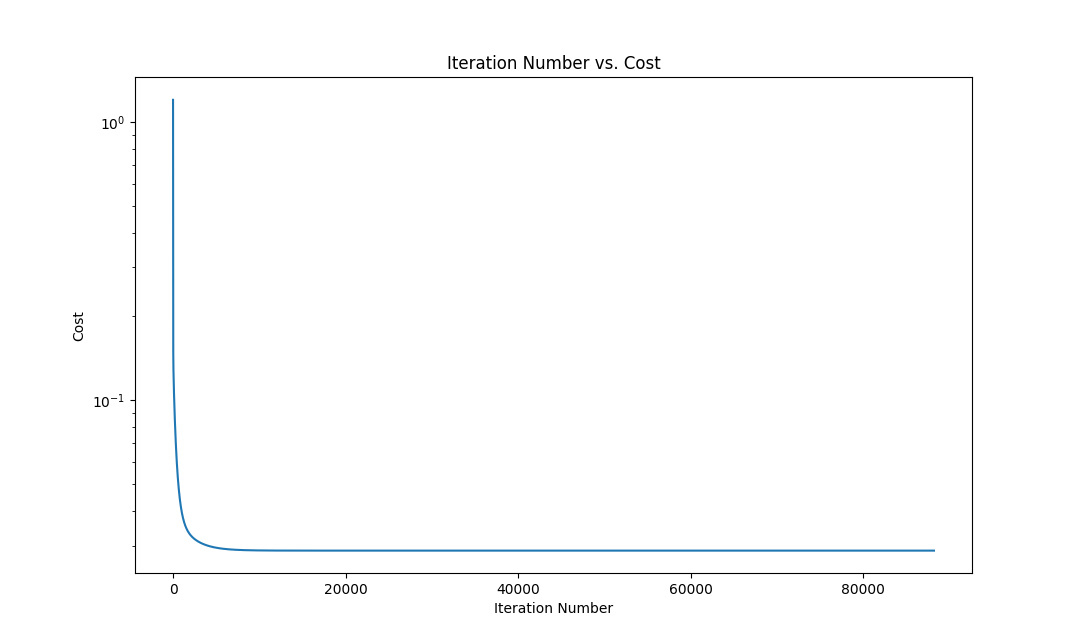
\includegraphics[width=1\textwidth]{cost.png}
\end{figure}

To see how accurate my predictions were visually, I plotted a point for each text: one point that represented the predicted WPM Ratio from my equation and one point that represented the actual WPM Ratio for that text. When plotting this graph, I sorted all the texts by their WPM Ratio so that it's easier to see how my prediction function compares against the actual values:

\begin{figure}[H]
	\caption{A graph of text number vs. WPM Ratio. The orange dots represent predictions from my prediction function and the green dots represent the actual WPM Ratio values of a word.}
	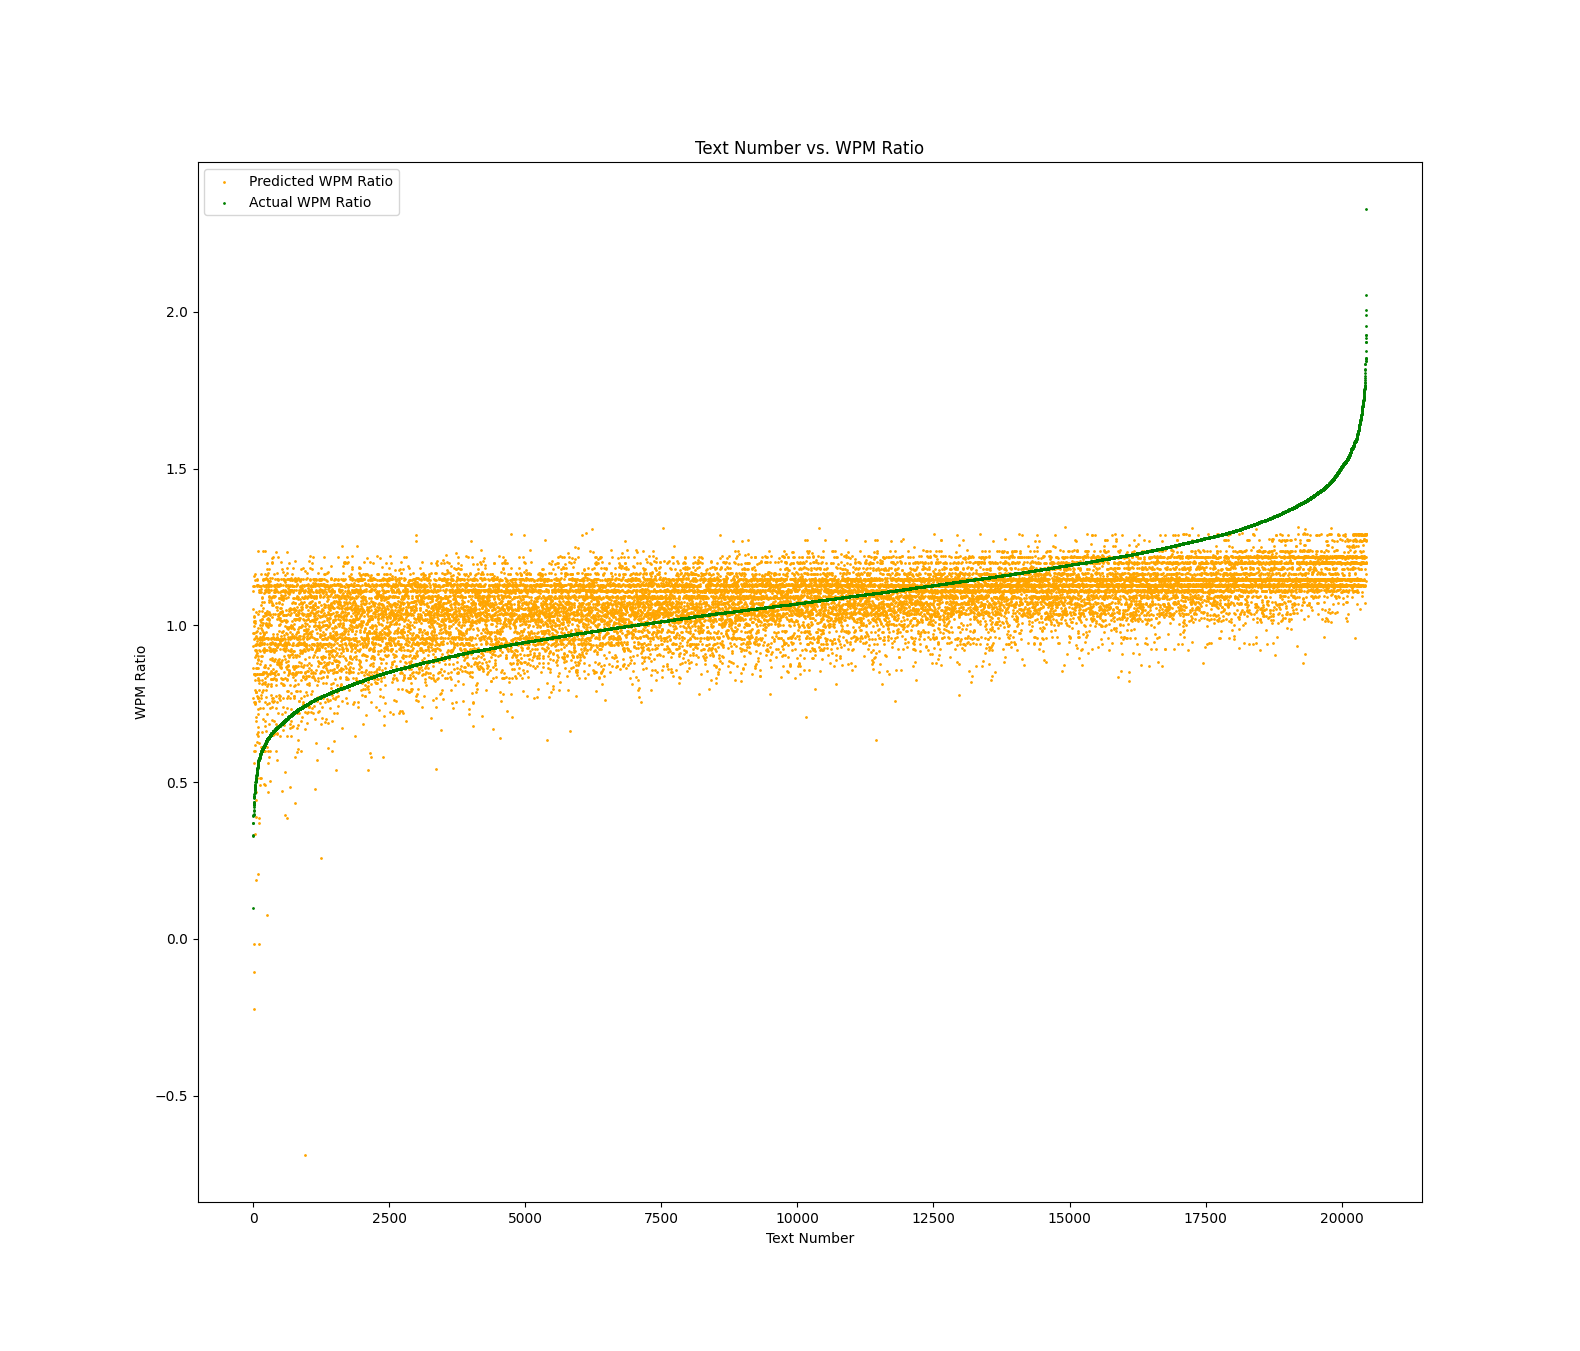
\includegraphics[width=\textwidth]{predictions.png}
\end{figure}

The general pattern of the predicted WPM ratios matches the general pattern of the graph: as the actual WPM ratios increase, the predicted WPM ratios also tend to increase. However, there is a lot of deviation between the predicted WPM ratio and the actual WPM ratio, indicating that there are likely more factors that influence typing speed that I haven't taken into account.

On the left side of the graph in Figure 10, there are a lot more predictions that match up with the low WPM ratio values. However, on the right side of the graph, there are fewer predictions that accurately predict the high WPM ratio values. This indicates that my prediction function is better at predicting the typing speed for difficult words, but worse at predicting the typing speed for easier words.

\section*{Creating the WPM Prediction Program}

My prediction function $f$ tells me how fast I can type a single word, but I want to create a program that can tell me how fast I would be able to type an entire text that consists of multiple words.

Luckily, I can use my prediction function to output a predicted WPM ratio for each word, and I can combine the WPM ratio of each word in the text to arrive at a final WPM prediction for the entire text.

The WPM of an entire text is calculated by the number of words in the phrase (and since a word is defined as 5 characters, it's equivalent to one-fifth the number of characters in the text) divided by the minutes it takes to type. It's easy to find the number of characters in the text, so I just need to find how long it would take for me to type the text based using the outputs of my prediction function $f$.

Since the prediction function only works on words, we can apply the prediction function on each word in the text. Then, we can convert the WPM ratio for each word into how long it would take for me to type the word using the following equations:
\begin{align*}
	f(\text{Word}_i)                                                                    & = \text{WPM Ratio}_i
	\\
	\text{WPM Ratio}_i * \text{Average WPM}                                             & = x~\frac{\text{words}}{\text{minute}}
	\\
	x~\frac{\text{words}}{\text{minute}} \times 5 \frac{\text{characters}}{\text{word}} & = 5x \frac{\text{characters}}{\text{minute}}
	\\
	                                                                                    & = \frac{1}{5x} \frac{\text{minutes}}{\text{character}}
	\\
	\text{\# minutes to type}~\text{Word}_i = m_i                                       & = \frac{1}{5x} * Length(\text{Word}_i)
\end{align*}

Then, we can add the value of $m_i$ for each word in the text to find the predicted total number of minutes to type the entire text. By combining this with the number of words in the text, we can calculate the predicted WPM of typing the entire text:
\begin{align*}
	\text{Total minutes to type text} & = \sum_{i=1}^{\text{\# of words}} m_i
	\\
	\text{\# words in text}           & = \frac{Length(\text{Word}_i)}{5}
	\\
	\text{WPM of Text}                & = \frac{\text{Total minutes to type text}}{\text{\# words in text}}
\end{align*}

To test the accuracy of my prediction function on entire texts, I applied the above formula to predict the WPM of all texts that I typed in TypeRacer with 100\% accuracy (the texts need to have 100\% accuracy as I didn't take accuracy into account when designing the machine learning model):

\begin{figure}[H]
	\caption{The predicted WPM using my prediction function $f$ compared with the actual WPM of the races.}
	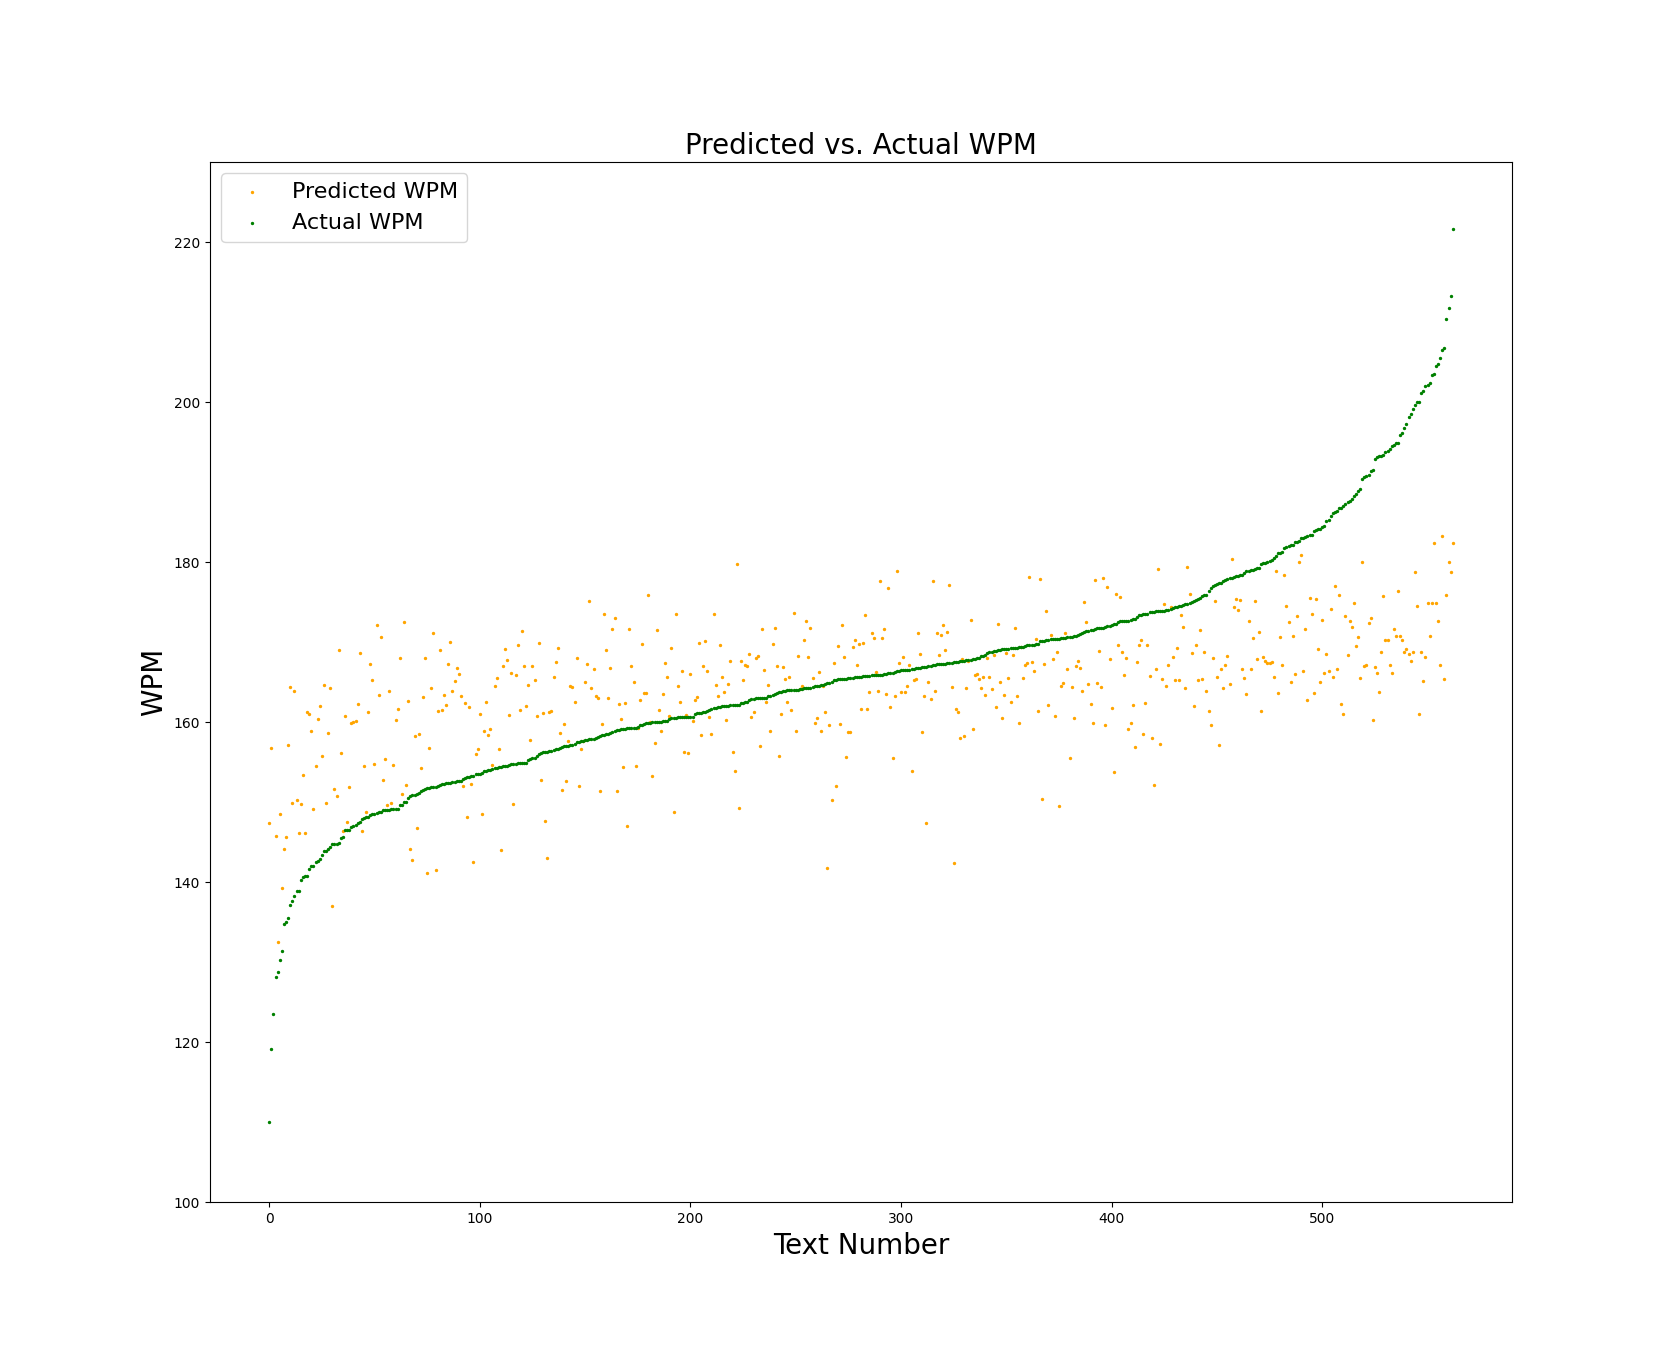
\includegraphics[width=\textwidth]{predicted-vs-actual-wpm.png}
\end{figure}

While there is a lot of variation in the graph, the WPM predictions do tend to increase as the actual WPM scores increase. This indicates that, overall, my prediction function was able to correlate certain text features with easier texts and other text features with difficult texts and produce a somewhat accurate WPM prediction based on these text features.

\section*{Conclusion}

In conclusion, I was able to successfully create a machine learning algorithm that correlated certain text features with making the text easier to type and certain text features with making the text harder to type. While the machine learning algorithm wasn't the most accurate with its predictions (i.e. there was a lot of deviations), its predictions did manage to follow the general trend: on average, as the actual WPM ratios increased, the predicted WPM ratios increased as well.

Even though I would consider my machine learning model generally successful, there is still much room for improvement. There are many more features affecting the typing speed of words that I didn't get to analyze in this exploration, such as the impact of words involving alternating hands and ``finger rolls'' that involve pressing a series of adjacent keys with different fingers in quick succession. In addition, many of these features aren't necessarily linearly correlated, which would change my prediction function $f$ and my cost function $C$. However, even with these changes, I would still be able to apply gradient descent to these new functions as long as I can calculate the derivative of these non-linear correlations.

Overall, I'm very proud of implementing my very first machine learning algorithm, especially using a data set that came from my own activity over the past 5 years of playing TypeRacer (who knew it would end up becoming immensely valuable for a math exploration?). I hope to apply machine learning to analyze various data from other parts of my life in the future.

\newpage

\section*{Works Cited}

\nocite{*}
\setlength\bibitemsep{1.5\itemsep}
\printbibliography

\newpage